% !TeX root = main.tex
\section{Results}
\label{Results}
Resulting from the work are the squared l2 euclidean distances calculated with the program OpenFace. The distance shows the similiarity to the given biometric references, it is a dissimilarity score. A lower distance means the compared two biometric references are more equal, when the distance is under a given threshold, these two biometric references are accepted to be the same biometric reference and so access is given. The resulting morphed photos were compared to diffrent photos of both biometric references, to get a independend distance. Which percentage of each biometric reference and the picture number is shown in \ref{percentageMorph}.
\subsection{Distances}

\subsubsection{Subset of 5 automatic generated morph sets (from biometric references also used by Budrhani)}\label{sec:subset5}
\todo{Vllt. sollten wir die Überschrift ändern - Wer ist Budrhani?}
All resultingsquared l2 euclidean distances for the morphed photos of biometric references 01-m-002-27 to 01-m-003-24, 01-m-003-24 to 01-m-005-23, 01-m-004-23 to 01-m-005-23, 01-m-010-23 to 01-m-013-23 and 01-m-014-23 to 01-m-016-23 compared to the corresponding compare images are way too much data. So there is as an example of the morphed image 01-m-002-27 - 01-m-003-24:

\begin{tabular}{lrrrrrr}
	Picture & 01-m-002-28 & 01-m-002-29 & 01-m-002-30 & 01-m-003-25 & 01-m-003-26 & 01-m-003-27 \\
	 & & & & & & \\
	1 & 0.11916 & 0.07499 & 0.19188 & 1.30874 & 1.16709 & 1.31322\\
	2 & 0.13701 & 0.06885 & 0.18756 & 1.25716 & 1.10248 & 1.25841\\ 
	3 & 0.17384 & 0.06523 & 0.19060 & 1.17656 & 1.01354 & 1.17311\\ 
	4 & 0.22901 & 0.07982 & 0.21253 & 1.08009 & 0.90457 & 1.06856\\ 
	5 & 0.31766 & 0.12439 & 0.24763 & 0.89989 & 0.70834 & 0.88006\\ 
	6 & 0.39700 & 0.16766 & 0.30990 & 0.83492 & 0.62518 & 0.81035\\ 
	7 & 0.50975 & 0.24823 & 0.40167 & 0.72848 & 0.51501 & 0.70676\\ 
	8 & 0.67400 & 0.39087 & 0.53792 & 0.60985 & 0.39251 & 0.59632\\ 
	9 & 0.74737 & 0.46525 & 0.58010 & 0.52552 & 0.32146 & 0.50314\\ 
	10 & 0.94108 & 0.62628 & 0.74969 & 0.40924 & 0.21060 & 0.37129\\ 
	11 & 1.05918 & 0.76321 & 0.86483 & 0.32472 & 0.13804 & 0.28219\\ 
	12 & 1.21209 & 0.90143 & 0.99503 & 0.25177 & 0.08833 & 0.20977\\ 
	13 & 1.25246 & 0.97993 & 1.05583 & 0.19876 & 0.05832 & 0.17236\\ 
	14 & 1.34758 & 1.07654 & 1.14637 & 0.19252 & 0.04679 & 0.16232\\ 
	15 & 1.37122 & 1.13813 & 1.18339 & 0.14941 & 0.05522 & 0.13605\\ 
\end{tabular}\\

Also shown in figure \ref{fig:Result1}.

The results of the 01-m-002-27 to 01-m-003-24, 01-m-003-24 to 01-m-005-23, 01-m-004-23 to 01-m-005-23, 01-m-010-23 to 01-m-013-23 and 01-m-014-23 to 01-m-016-23 morphs are shown in figure \ref{fig:Result1-5}.

For better recognizability the mean value of all the diffrent squared l2 euclidean distances is calculated for biometric reference 1 and biometric reference 2. The result is shwon in figure \ref{fig:Result1-5-mean}. The distance graphs crosses by ($9.04$, $0.49$), so the best distance for both biometric references is with picture 9 with distances of $0.48$ and $0.49$. Picture 9 with $42.86$\% of biometric reference 1 and $57.14$\% of biometric reference 2 so it  not the middle of all 15 pictures, this could be the cause of the different distances of the biometric references to their own compare images.

OpenFace uses normally a threshold of \textbf{$0.99$}, which allows nearly all morphs from picture 5 to 10 to be successful acknowledged as shown in figure \ref{fig:Result1-5}. Only in 3 cases there is the distance way too high to work properly. The compare pictures are 01-m-016-24.jpg, 01-m-016-25.jpg and 01-m-016-26.jpg which are all from the same biometric reference, so this morph with this biometric reference is not working, this could be the cause of the different distances to the own compare images. As a result in 4 out of 5 cases it is possible to morph two biometric references to be successful acknowledged, this makes a success chance of $80$\%.

\begin{figure}[htbp] 
	\centering
		\includegraphics[width=0.95\textwidth]{Resources/result1ODF.eps}
	\caption{Squared l2 euclidean distances (y axis) of morphs from 01-m-002-27 to 01-m-003-24 (with 15 steps ont he x axis) comparing to 01-m-002-28.jpg, 01-m-002-29.jpg, 01-m-002-30.jpg, 01-m-003-25.jpg, 01-m-003-26.jpg and 01-m-003-27.jpg}
	\label{fig:Result1}
\end{figure}

\begin{figure}[htbp] 
	\centering
		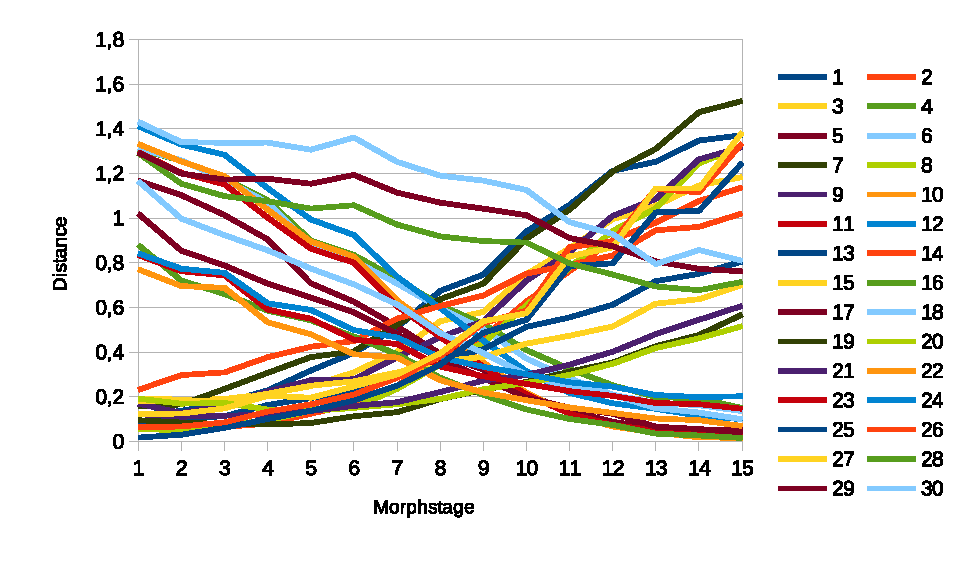
\includegraphics[width=0.95\textwidth]{Resources/result1-5ODF.eps}
	\caption{Squared l2 euclidean distances (y axis) of morphs from 01-m-002-27 to 01-m-003-24, 01-m-003-24 to 01-m-005-23, 01-m-004-23 to 01-m-005-23, 01-m-010-23 to 01-m-013-23 and 01-m-014-23 to 01-m-016-23 (with 15 steps on the x axis) comparing to the corresponding compare photos}
	\label{fig:Result1-5}
\end{figure}

\begin{figure}[htbp] 
	\centering
		\includegraphics[width=0.95\textwidth]{Resources/result1-5-meanODF.eps}
	\caption{Mean squared l2 euclidean distances (y axis) of morphs from 01-m-002-27 to 01-m-003-24, 01-m-003-24 to 01-m-005-23, 01-m-004-23 to 01-m-005-23, 01-m-010-23 to 01-m-013-23 and 01-m-014-23 to 01-m-016-23 (with 15 steps on the x axis) comparing to the corresponding compare photos}
	\label{fig:Result1-5-mean}
\end{figure}
\newpage
\subsubsection{Subset of 39 automatic generated morph sets}\label{sec:subset39}
Now 39 automatic generated sets of morphed biometric references were used. The used biometric references are:
\begin{multicols}{3}
\begin{itemize}
\item 01-m-002 - 01-m-003
\item 01-m-003 - 01-m-004
\item 01-m-004 - 01-m-005
\item 01-m-013 - 01-m-014
\item 01-m-016 - 01-m-017
\item 01-m-019 - 01-m-020
\item 01-m-020 - 01-m-021
\item 01-m-021 - 01-m-022
\item 01-m-022 - 01-m-023
\item 01-m-025 - 01-m-026
\item 01-m-026 - 01-m-027
\item 01-m-030 - 01-m-031
\item 01-m-031 - 01-m-032
\item 01-m-032 - 01-m-033
\item 01-m-037 - 01-m-038
\item 01-m-038 - 01-m-039
\item 01-m-039 - 01-m-040
\item 01-m-040 - 01-m-041
\item 01-m-041 - 01-m-042
\item 01-m-042 - 01-m-043
\item 01-m-043 - 01-m-044
\item 01-m-044 - 01-m-045
\item 01-m-045 - 01-m-046
\item 01-m-046 - 01-m-047
\item 01-m-047 - 01-m-048
\item 01-m-048 - 01-m-049
\item 01-m-051 - 01-m-052
\item 01-m-052 - 01-m-053
\item 01-m-053 - 01-m-054
\item 01-m-054 - 01-m-055
\item 01-m-055 - 01-m-056
\item 01-m-059 - 01-m-060
\item 01-m-060 - 01-m-061
\item 01-m-065 - 01-m-066
\item 01-m-066 - 01-m-067
\item 01-m-069 - 01-m-070
\item 01-m-072 - 01-m-073
\item 01-m-073 - 01-m-074
\item 01-m-074 - 01-m-075
\end{itemize}
\end{multicols}


With these sets again the squared l2 euclidean distances are computed to the associated compare images of the two biometric references. The resulting distances are shown in figure \ref{fig:Result39-all}. To decrease the amount of information the mean values for both biometric references were computed and are shown in figure \ref{fig:Result39-mean}. The distance graphs crosses by ($7.93$, $0.6$), so the best distance for both biometric references is with picture 8 with distances of $0.6$ and $0.59$. Picture 8 is the exact middle of all 15 pictures with $50$\% of biometric reference 1 and $50$\% of biometric reference 2.
\begin{figure}[htbp] 
	\centering
		\includegraphics[width=0.95\textwidth]{Resources/result39-allODF.eps}
	\caption{Squared l2 euclidean distances (y axis) of the subset of 39 morphs (with 15 steps on the x axis) comparing to the corresponding compare photos}
	\label{fig:Result39-all}
\end{figure}
\begin{figure}[htbp] 
	\centering
		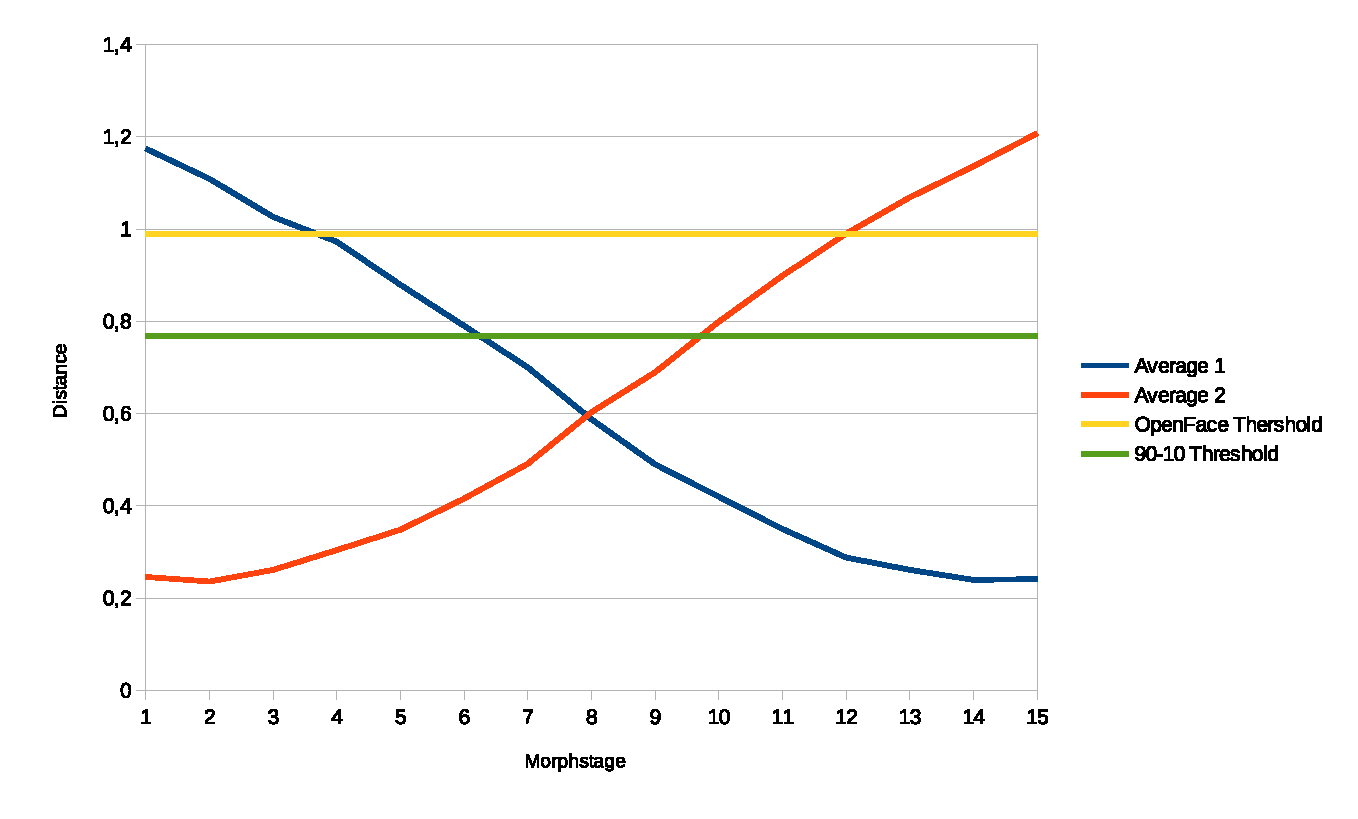
\includegraphics[width=0.95\textwidth]{Resources/result39-meanODF.eps}
	\caption{Mean squared l2 euclidean distances (y axis) of the subset of 39 morphs (with 15 steps on the x axis) comparing to the corresponding compare photos}
	\label{fig:Result39-mean}
\end{figure}

\newpage
\subsubsection{Subset of 8 manual generated morph sets}
\label{sec:subsetman}
Finally 8 sets of morphed biometric references were created and the distances to the comparing images was calculated. As a speciality in this set a morph of a woman and a man.
The biometric references for the manual morphing are:
\begin{multicols}{2}
\begin{itemize}
\item 01-m-002-27 - 01-m-003-24
\item 01-m-003-24 - 01-m-005-23
\item 01-m-004-23 - 01-m-005-23
\item 01-m-010-23 - 01-m-013-23
\item 01-m-014-23 - 01-m-016-23
\item 01-m-017-23 - 01-m-019-23
\item 01-m-020-23 - 01-w-002-23
\item 01-w-036-23 - 01-w-037-23
\end{itemize}
\end{multicols}
For this subset the squared l2 euclidean distances to the associated compare images of the two biometric references is also computed. The resulting distances are shown in figure \ref{fig:result-jannis-all}. To decrease the amount of information the mean values for both biometric references were computed and are shown in figure \ref{fig:result-jannis-mean}.

\begin{figure}[htbp] 
	\centering
		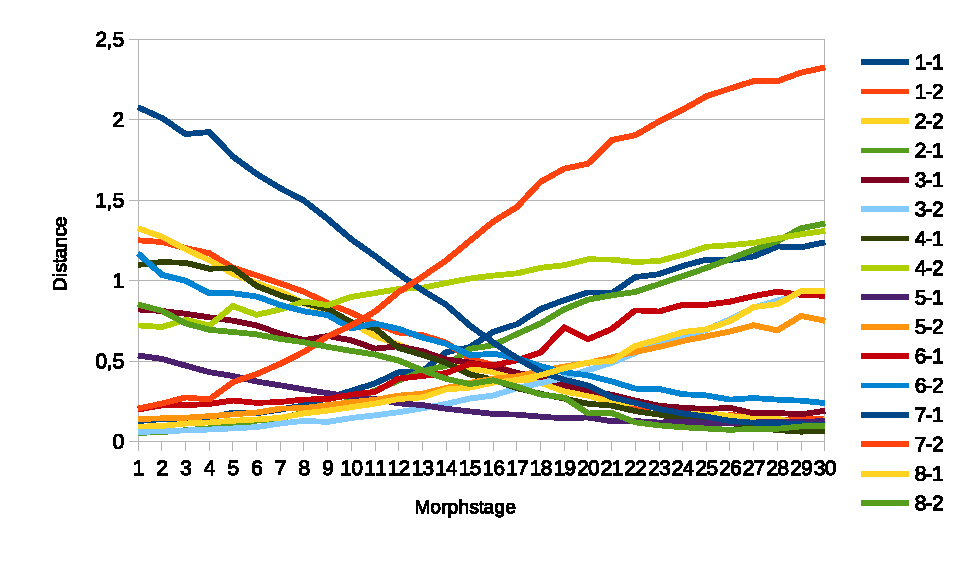
\includegraphics[width=0.95\textwidth]{Resources/result-jannisODF.eps}
	\caption{Squared l2 euclidean distances (y axis) comparing to the corresponding compare photos of the subset of 8 manual morphs (with 30 steps on the x axis)}
	\label{fig:result-jannis-all}
\end{figure}
\begin{figure}[htbp] 
	\centering
		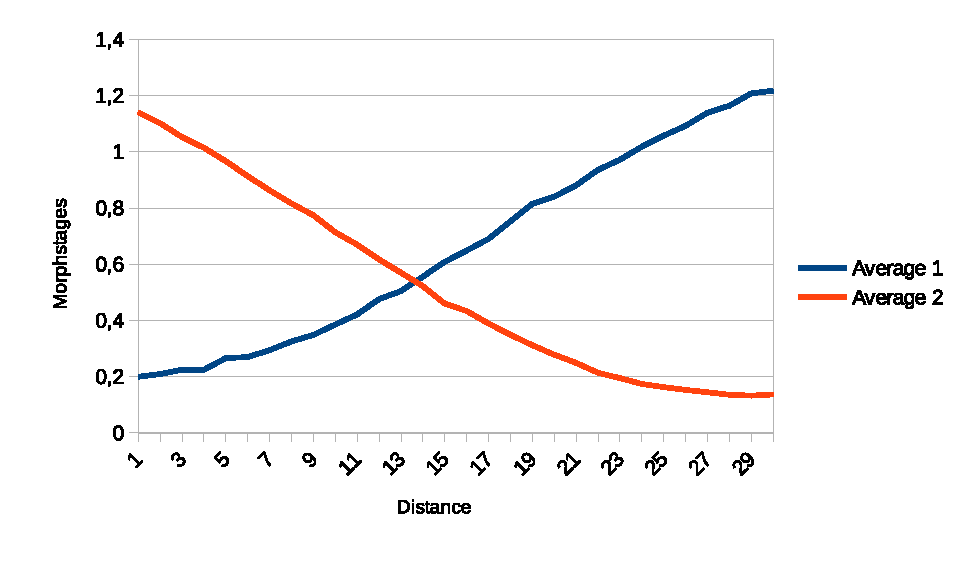
\includegraphics[width=0.95\textwidth]{Resources/result-jannis-meanODF.eps}
	\caption{Mean squared l2 euclidean distances (y axis) comparing to the corresponding compare photos of the subset of 8 manual morphs (with 30 steps on the x axis)}
	\label{fig:result-jannis-mean}
\end{figure}

%\newpage
\subsection{Threshold}
\label{Threshold}
As a result a threshold is computed to get a $10$\% biometric false acceptance of an impostor (false match rate (FMR)) and a $90$\% chance to non-match a morphed image.

\subsubsection{Automatic morphing (Subset of 39 automatic generated morph sets)}\label{sec:automorph-thres}
For the calculation of the threshold of the automatic generated morphs the subset of 39 of section \ref{sec:subset39} is used, it's bigger than the subset of 5 automatic generated morph sets (from biometric references also used by Budrhani) of section \ref{sec:subset5} so the used mean values are more representative.
Used for the calculation are the squared l2 euclidean distances of section \ref{sec:subset39}.
The resulting threshold for this subset is \textbf{$0.76891524$}. In contrast to the distances it is shown in figure \ref{fig:Result39-90-10}.


\begin{figure}[htbp] 
	\centering
		\includegraphics[width=0.95\textwidth]{Resources/result39-90-10ODF.eps}
	\caption{Squared l2 euclidean distances (y axis) of the 39 morphed subset (with 15 steps on the x axis) compared to the corresponding compare photos, in contrast to the calculated threshold of $0.76891524$} %\todo{beschreibung anpassen}
	\label{fig:Result39-90-10}
\end{figure}

\subsubsection{Manual morphing (Subset of 8 manual generated morph sets)}\label{sec:manmorph-thres}
For the calculation of the threshold of the manual generated morphs the subset of 8 of section \ref{sec:subsetman} is used and the calculated distances from the same section.
The resulting threshold for this subset is \textbf{$0.7172467154$}. In contrast to the distances it is shown in figure \ref{fig:Resultman-90-10}.


\begin{figure}[htbp] 
	\centering
		\includegraphics[width=0.95\textwidth]{Resources/result-jannis-mean-90-10ODF.eps}
	\caption{Squared l2 euclidean distances (y axis) of the 8 manual morphed subset (with 30 steps on the x axis) compared to the corresponding compare photos, in contrast to the calculated threshold of $0.7172467154$} %\todo{beschreibung anpassen}
	\label{fig:Resultman-90-10}
\end{figure}

\subsubsection{Comparison threshold of manual and automatic}\label{sec:comp-thres}
The two tresholds of the automatic morphing from \autoref{sec:automorph-thres} $0.76891524$ and the manual morphing in \autoref{sec:manmorph-thres} $0.7172467154$ are close to another. They differ only about $0.05$, which is not much. The threshold of the manual morphing is lower than the automatic threshold, this could mean that the images of the manual morphing are better, but such a low difference could also be possible through lower the distances because of the input biometric reference variations.

As a result the threshold of OpenFace should be set to $0.71$ to fight off morphing attacks, in fact the biometric false rejection rate in the biometric system is acceptable.

\todo[inline]{Compare to threshold of other papers: Suggestion: Compared to \cite{ferrara2014magic} which is based on \cite{baltruvsaitis2016openface} (threshold of 0.999) we were able to show that a 90-10 threshold is already achieved at a much lower distance. }